
Having written a completely general program, we are free to add as many
celestial objects as we'd like. However, we start by looking at the Sun-Earth
system in order to test the stability of our program as function of time step
$\D t$.

In approximating Earth's orbit around the Sun as circular, we obtained our
mass units. We apply Newton's 2nd law and his gravitational law to find at which
velocity the orbit is circular.
%
\begin{align*}
	F_G &= M_{\text{Earth}}a \\
	G \frac{M_{\odot}M_{\text{Earth}}}{r^2} &= M_{\text{Earth}}a
\end{align*}
%
For circular orbits we can write the acceleration as
%
\begin{equation*}
	a = \frac{v^2}{r}
\end{equation*}
which gives us
%
\begin{align*}
	v^2 &= G \frac{M_{\odot}}{r^2} \\
	v &= \sqrt{ \frac{GM_{\odot}}{r^2}}
\end{align*}
%
Inserting $GM_{\odot} = 4\pi^2$, $r = 1$ AU, we get
%
\begin{equation*}
	v = 2\pi
\end{equation*}
%
We place the Sun at the origin, with Earth at a distance 1 AU in $x$-direction.
Earth's velocity $v$ is initially directed in the $y$-direction. The orbit
around the Sun is shown in figure \refig{sunEarth-dt0.01}.
%
\begin{figure}[htpb]
	\centering
	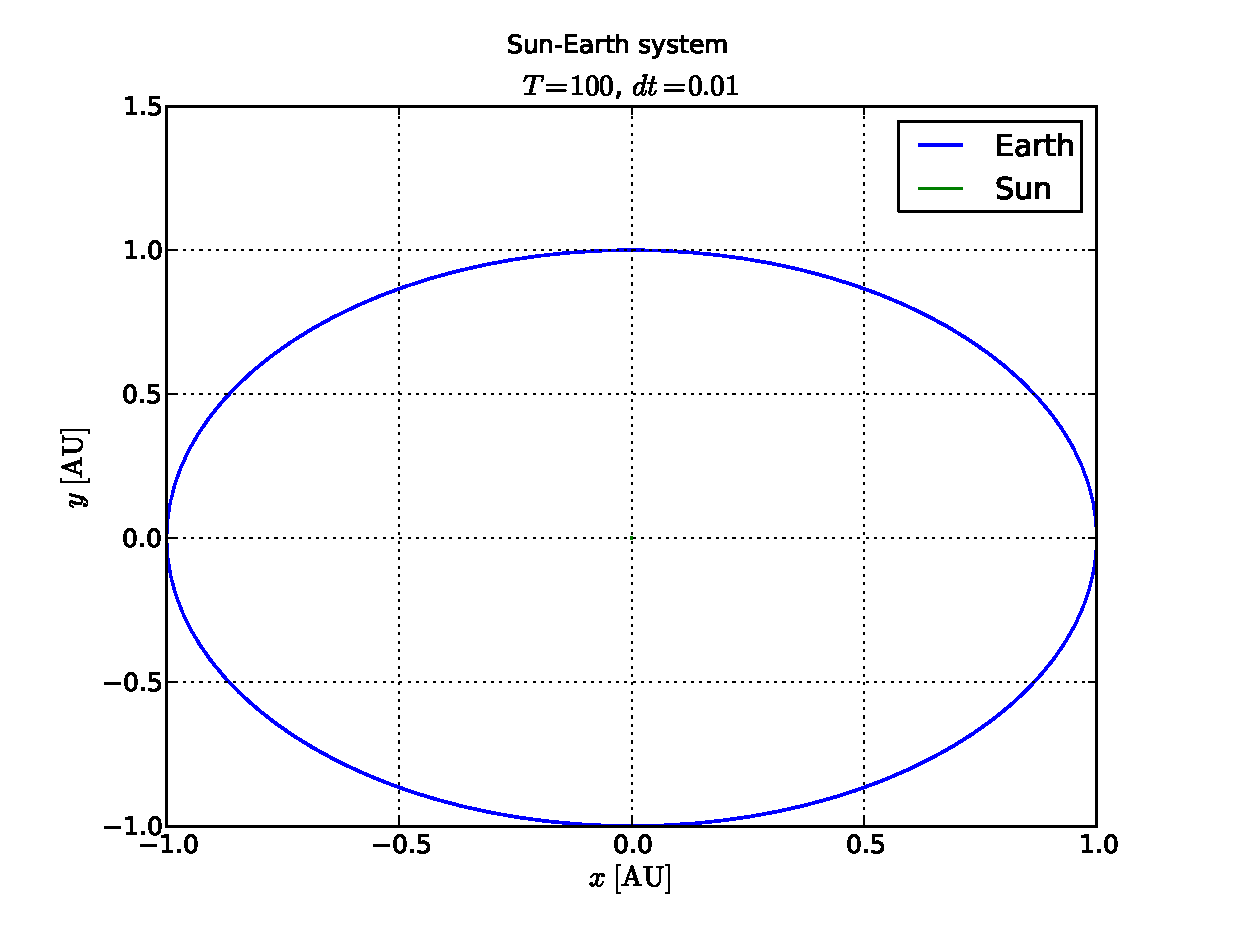
\includegraphics[width=0.8\textwidth]{figures/sun_earth_T100_dt1e-2}
	\caption{Earth's circular orbit around the Sun over a period of $T = 100$
	 years, with time step $\D t = 0.01$. The initial values are
	 $\mathbf{r} = [1,0]$, $\mathbf{v} = [0,1]$.}
	\label{fig:sunEarth-dt0.01}
\end{figure}
%
We notice that the orbit is circular (notice the axes), as expected, and quite
stable.
%By zooming far in on the center of Earth's orbit, we can see the
%movement of the Sun. See figure \refig{sun-zoom}.
%
%\begin{figure}[htpb]
%	\centering
%	\includegraphics[width=1.0\textwidth=]{figures/sun_zoom_dt1e-2.eps}
%	\caption{The Sun's movement due to the Earth. One semicircle is the Sun's
%	movement over the course of a year.}
%	\label{fig:sun-zoom}
%\end{figure}
%
Given that the orbit is circular, we expect the kinetic energy and the potential
energy to be conserved. The velocity is only expected to change its direction,
and not magnitude,
while orbiting, while the distance to the Sun is always the same. We can see
that this is the case in figure \refig{energycons}, which shows the energy
conservation.
%
\begin{figure}[htpb]
	\centering
	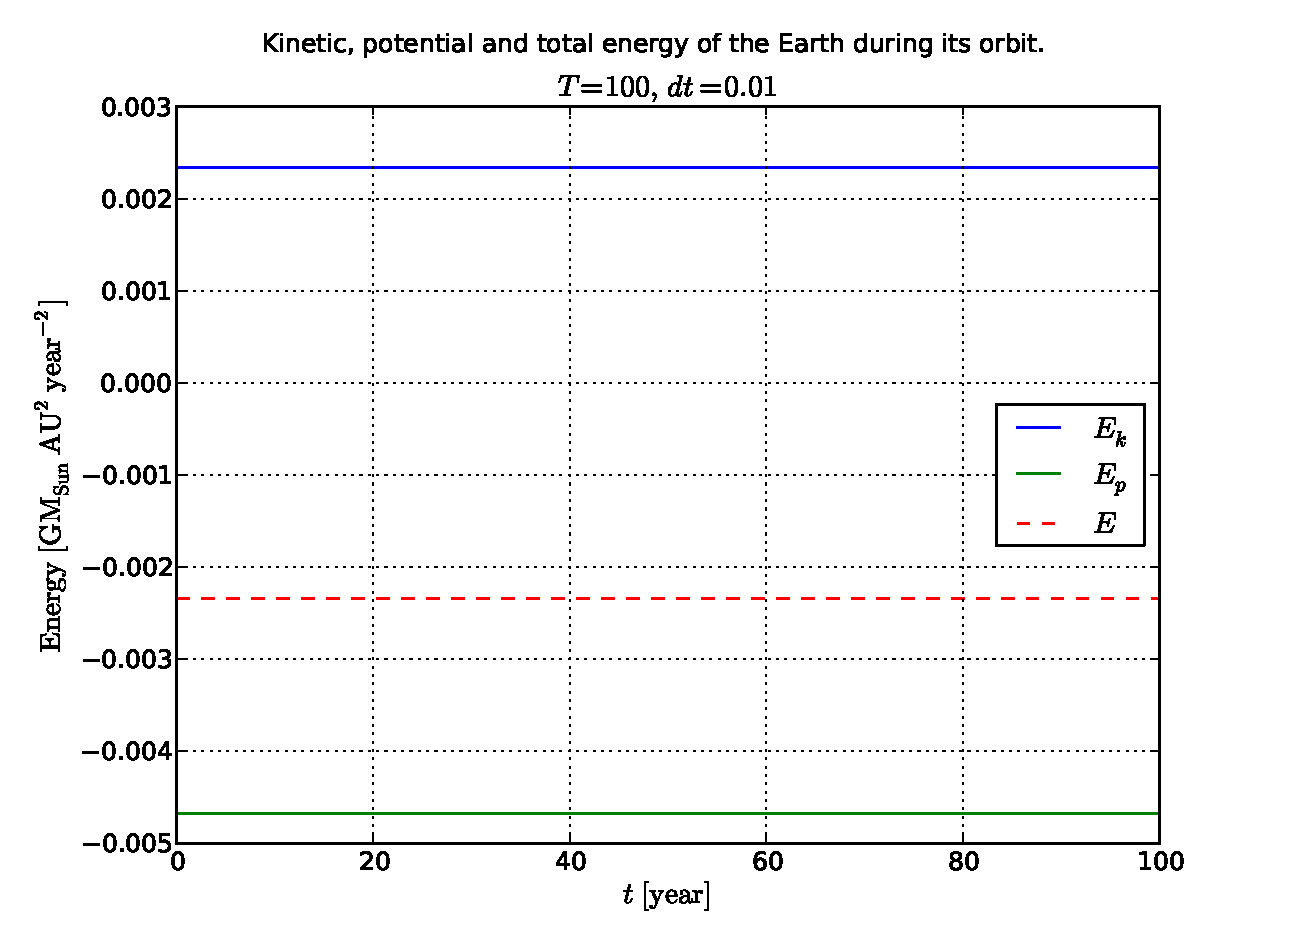
\includegraphics[width=0.8\textwidth]{figures/earth_energy_dt1e-2}
	\caption{The kinetic, potential and total energy of the Earth over a period
	of $T = 100$ years, with $\D t = 0.01$. We see that both energy forms are
	conserved.}
	\label{fig:energycons}
\end{figure}
%
The angular momentum $\mathbf{L}$ is defined by
\begin{equation*}
	\mathbf{L} = \mathbf{r} \times\mathbf{p}
\end{equation*}
%
The velocity vector is always orthogonal to the position vector, such that the
direction of $\mathbf{L}$ is orthogonal to the $xy$-plane at all times. The
magnitude of the angular momentum vector is just the product $L =
rvM_{\text{Earth}}$, where $r$, $v$ are the magnitudes of the position vector
and velocity vector, respectively. We have shown above that these are constant,
so we expect the angular momentum of the Earth to be constant. The result is
shown in figure \refig{angmom}.
%
\begin{figure}[htpb]
	\centering
	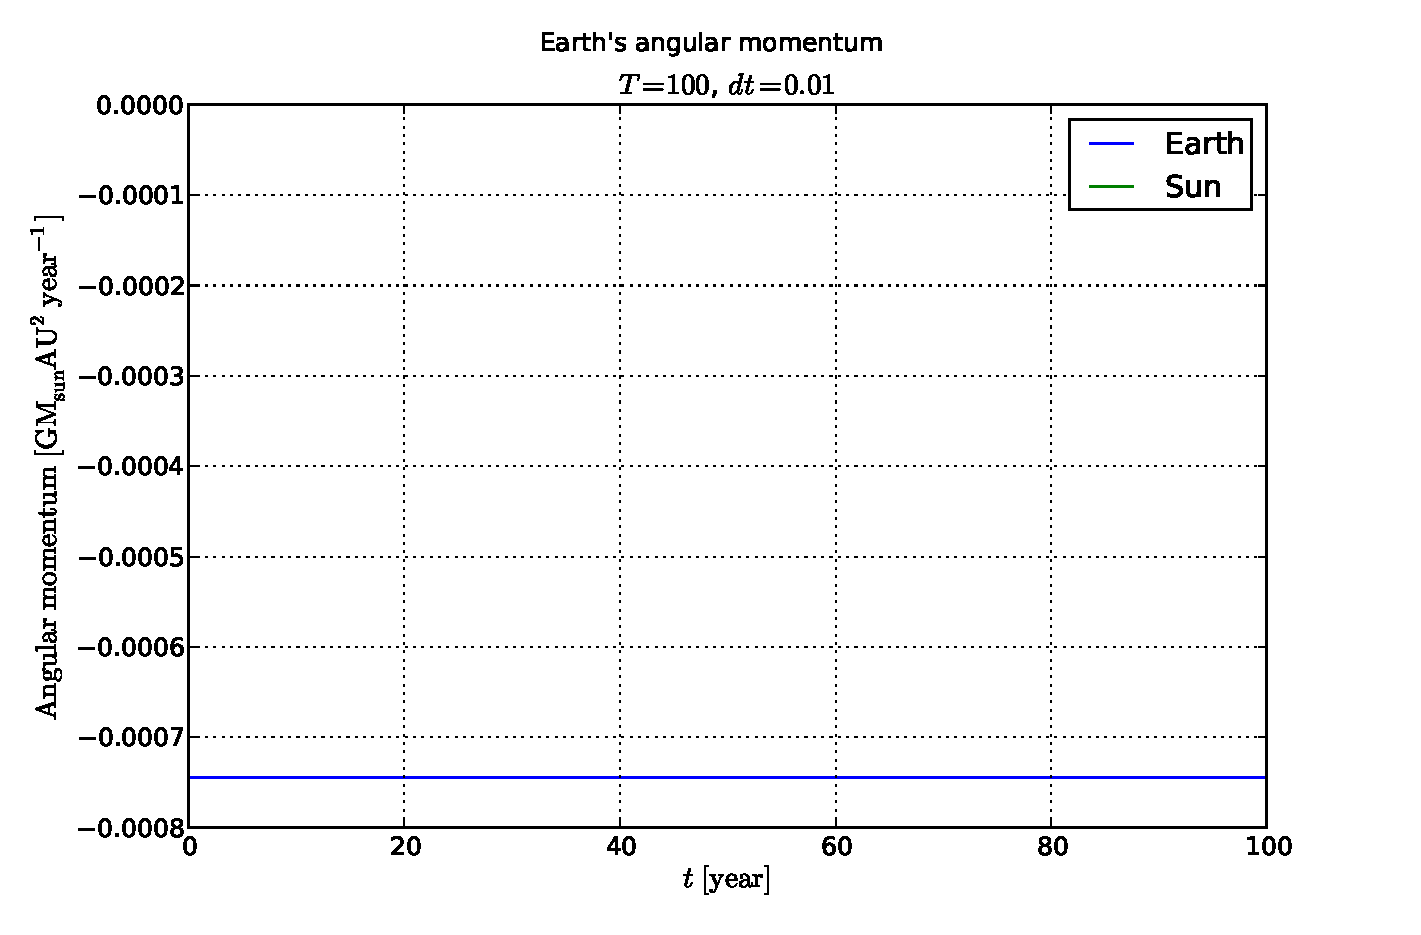
\includegraphics[width=0.8\textwidth]{figures/earth_angmom_dt1e-2}
	\caption{The angular momentum of the Earth, which is conserved throughout
	its orbit. Here shown for $T = 100$ years and $\D t = 0.01$.}
	\label{fig:angmom}
\end{figure}
%
Let us now see what happens when we increase the time step. We increase
$\D t$ by a factor of $10$, and consider Earth's orbit as shown in figure
\refig{sunEarth-dt0.1}.
%
\begin{figure}[htpb]
	\centering
	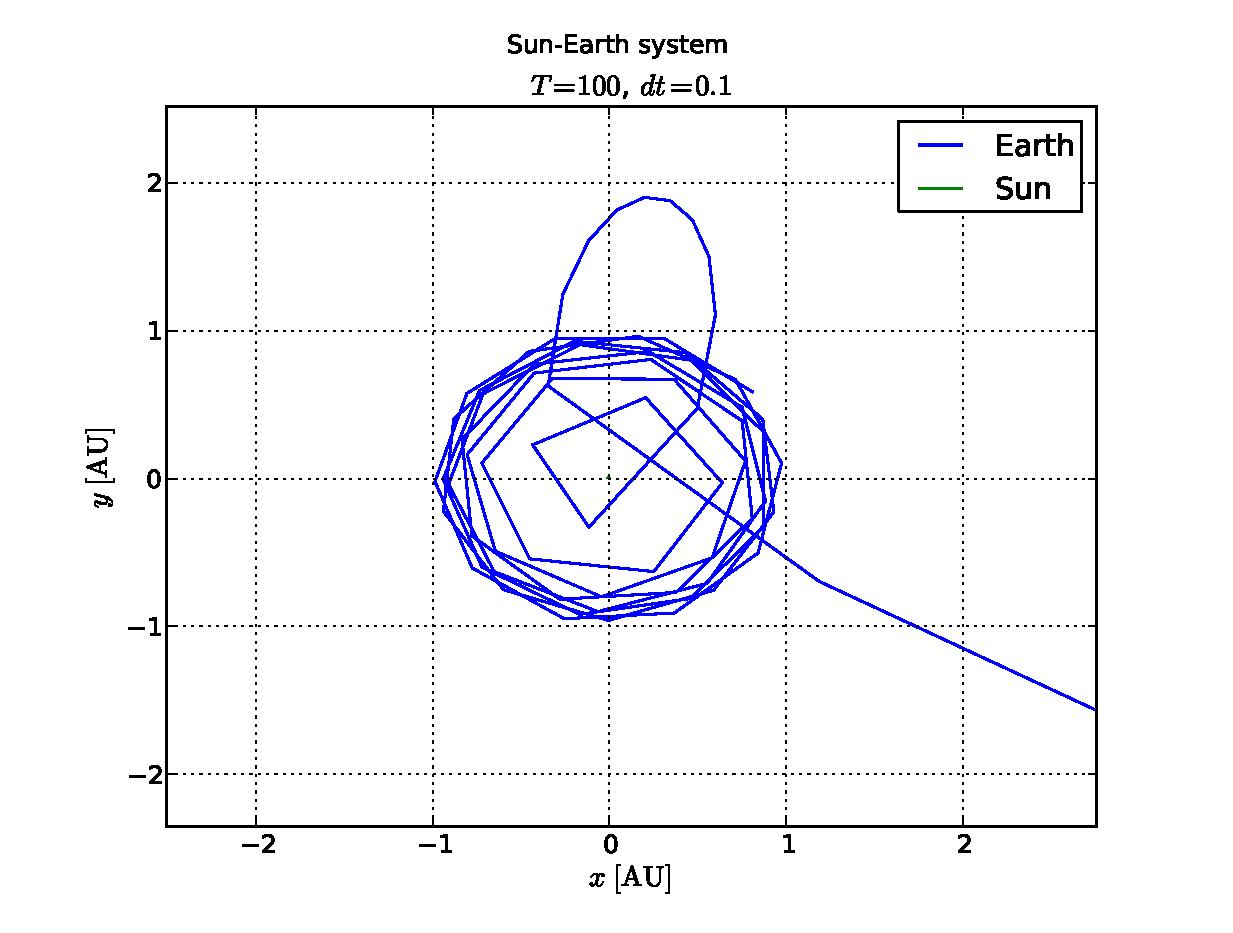
\includegraphics[width=0.8\textwidth]{figures/sun_earth_T100_dt1e-1_zoom}
	\caption{Earth's orbit around the sun for a time step $\D t = 0.01$. We have
	zoomed in on the original figure to better see what happens before the Earth
	leaves orbit.}
	\label{fig:sunEarth-dt0.1}
\end{figure}
%
The trajectory starts out in a rough circular orbit, but loses energy as it
completes several orbits. At one point it is much closer to the Sun, such
that it gathers a higher velocity, resulting in a half loop outside the original
orbit. Upon returning, it again gathers a velocity higher than the escape
velocity, such that it leaves the solar system. The energy plot for this orbit
is included as well. See figure \refig{energyconstdt0.1}.
%
\begin{figure}[htpb]
	\centering
	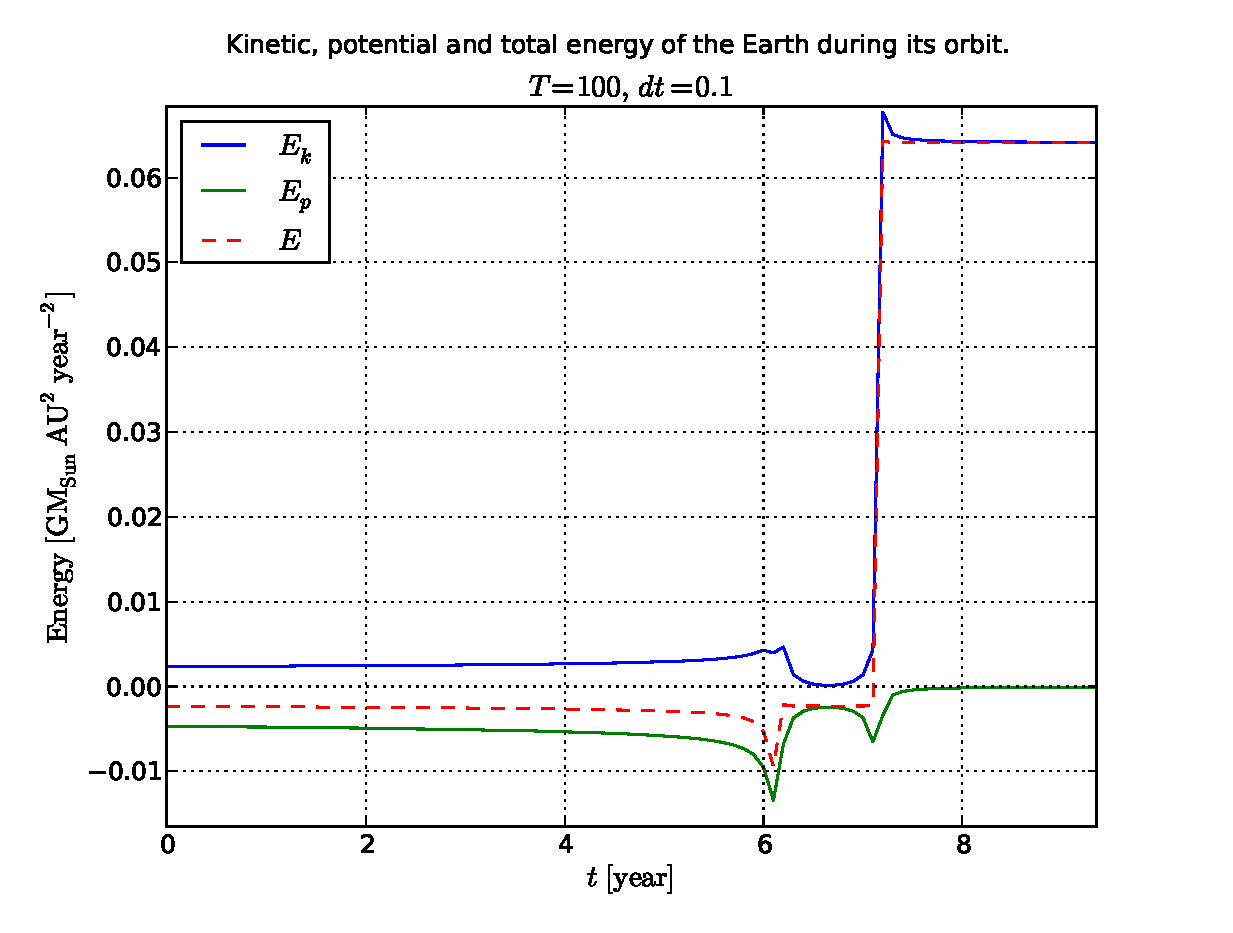
\includegraphics[width=0.8\textwidth]{figures/earth_energy_dt1e-1}
	\caption{Kinetic, potential and total energy for Earth while orbiting the
	Sun with time step $\D t = 0.1$, over a course of $T = 100$ years.
	We have zoomed in on the relevant area.}
	\label{fig:energyconstdt0.1}
\end{figure}
%
We see that the potential energy is approximately zero after $t = 8$ years,
which means that Earth is free of the Sun's gravitational pull after this
time. However the total energy have increased by an enormous amount.

This is obviously a flaw in the RK4 method. It doesn't conserve energy for any
time step $\D t$. Had we simulated the Sun-Earth system over a much longer time,
we would have seen the same thing happen for small time steps, like $\D t =
10^{-2}$. 
A time step $\D t = 0.1$ is big enough so that we can see the
method fail in the course of 100 years. We actually need less than 10 years
to see it fail, judging by figure \refig{energyconstdt0.1}. 
In some ways, a \emph{symplectic integrator} such as Euler-Cromer might have 
been better in such a simulation, because it conserves energy for any time step
$\D t$. Using Euler-Cromer instead would however have a negative effect on the
accuracy.

We can test how large $\D t$ can be before the method fails for a time span of 100
years. By trial and error we
find that a time step of about $\D t = 5.5 \cdot 10^{-2}$ is just small enough to
prevent failure. See figure \refig{sunEarth-dt5.5e-2}.
%
\begin{figure}[htpb]
	\centering
	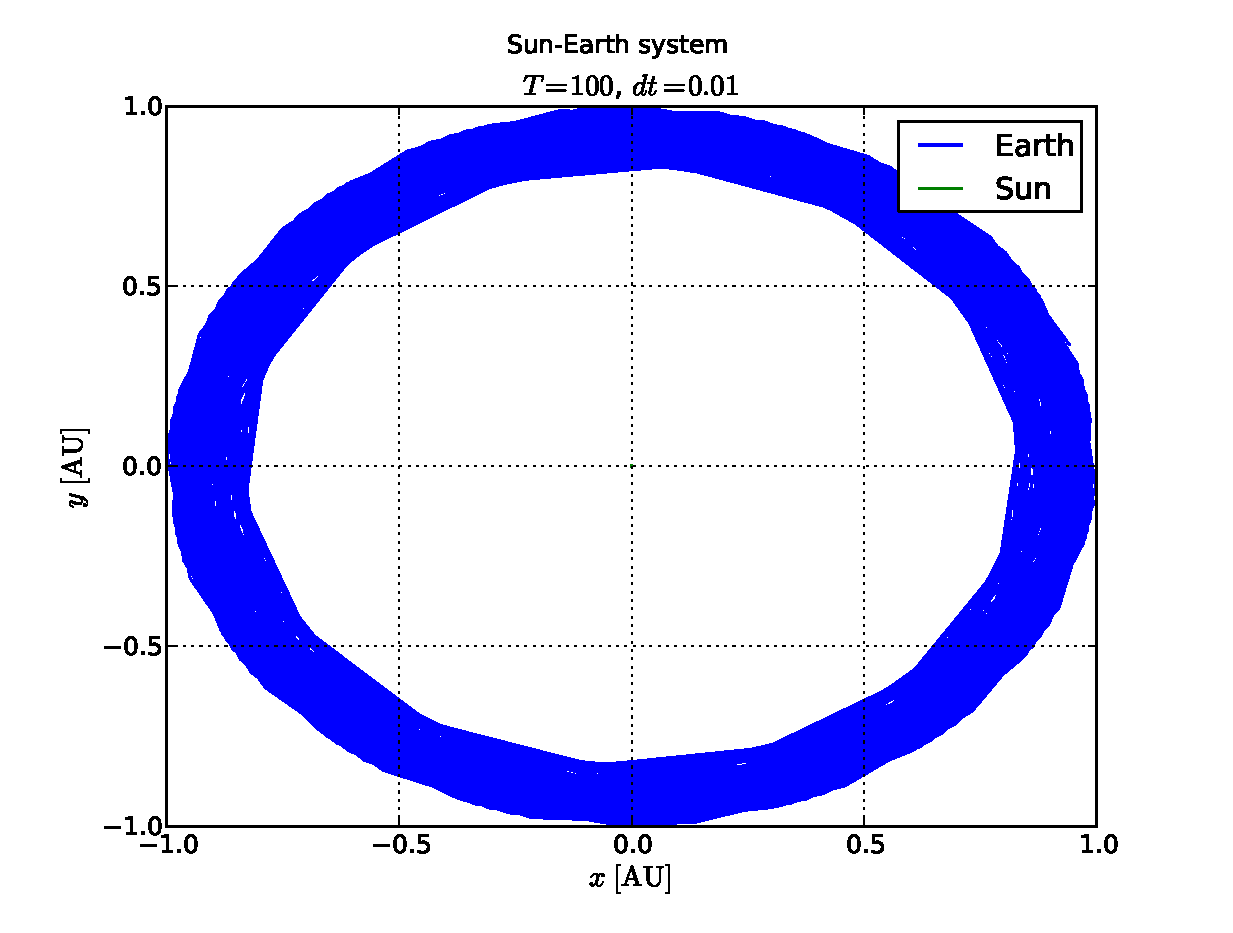
\includegraphics[width=0.8\textwidth]{figures/sun_earth_T100_dt5-5e-2}
	\caption{Earth's orbit about the Sun with $\D t = 5.5 \cdot 10^{-2}$. The
	method is on the verge of failing for this time step. This is only valid for
	$T < 100$ years.}
	\label{fig:sunEarth-dt5.5e-2}
\end{figure}
%
Had we increased the time step to $\D t = 6 \cdot 10^{-2}$, the method would have
failed. The limit then lies in the range $(5.5 - 6) \cdot 10^{-2}$.
